% vim: spelllang=en_au
\documentclass[a4paper]{article}

\usepackage{geometry}
\usepackage{amsmath}
\usepackage{enumerate}
\usepackage{amssymb}
\usepackage{amsthm}
\usepackage{hyperref}
\usepackage{minted}
\usepackage{enumitem}
% \usepackage[symbol]{footmisc}
\usepackage{tikz}
\usetikzlibrary{automata}
\usetikzlibrary{positioning,arrows.meta,calc}
\usetikzlibrary{angles,intersections,quotes,arrows.meta}

\author{Kait Lam \\ \small \texttt{45294583}}
\title{\textsc{Math3306} --- Assignment 1 (Submission)}
\date{16 August 2024}

\begin{document}

\maketitle


\section*{Question 1}
\begin{center}
  \textit{This question concerns deriving a FSA to recognise $L^*$, given a FSA to recognise $L$.}
\end{center}

\noindent First, we must (and so, we will)
introduce two language-preserving transformations on FSAs.
% \footnote{
%   That is, the transformation does not change the language recognised by the FSA.
% } transformations on FSAs.
% These will be useful later.
Assume we have a FSA given by $(Q, F, A, \tau, q_0)$ recognising a language $L$.
We introduce:
\begin{itemize}
  \item \textit{Unify accepting states.} It is possible to translate the FSA
    % into a form with a single accepting state and no
    into an equivalent\footnote{recognising the same language} FSA
    which has a single distinguished accepting state, and no outgoing edges from that accepting state.

    This is done by introducing a new symbol $\bullet^+$ with
    $\bullet^+ \notin Q$. We mark this as the only accepting state.
    Finally, for all edges \textit{into} a previously-accepting state, we
    duplicate those to point into $\bullet^+$.

    That is, the new equivalent FSA is
    \begin{align*}
      % (Q states, F final states, A alphabet, tau subset Q x A x Q, Q)
      (Q \cup \{\bullet^+\}, \{\bullet^+\}, A, \tau', q_0)
    % \end{align*}
      \qquad\text{where}~
    % \begin{align*}
      \tau' = \tau \cup
      \big\{(q, a, \bullet^+) \mid \exists q_F \in F.~ (q,a,q_F) \in \tau\big\}.
    \end{align*}
    
    To see that is is equivalent, note that we retain all previous states
    and transition edges, so it behaves identically for transitions which are not terminating.
    For edges handling the last character of a word and going into a
    previously-accepting state, note that the newly-added edges,
    $\tau' \setminus \tau$, will provide the option of moving to the accepting
    $\bullet^+$ state.
    $\bullet^+$ has no outgoing edges, and so will not accept more words than the original language.
    This is, of course, not a deterministic FSA.

  \item \textit{Distinct start state.}
    We can also translate the FSA into a form with a distinguished start state
    which is unreachable aside from the starting configuration.

    We introduce $\bullet^-$ with $\bullet^- \notin Q$ and mark this as the initial state.
    For all outgoing edges from the previous start state, we duplicate these onto $\bullet^-$. Importantly, we do not replicate incoming edges.

    Therefore, the 5-tuple is
    \begin{align*}
      (Q \cup \{\bullet^-\}, F, A, \tau', \bullet^-)
      \qquad\text{where}~
      \tau' = \tau \cup 
      \big\{(\bullet^-, a, q') \mid \exists q' \in Q.~ (q_0, a, q') \in \tau\big\}.
    \end{align*}
    We can see that $\bullet^-$ acts ``{just like}'' the previous $q_0$ for its
    start state behaviour, and the behaviour when $q_0$ is (potentially) revisited is retained by $q_0$ (since the transformation maintains $q_0 \in Q$).
    Thus, we claim it recognises precisely the same language.
\end{itemize}


Now, we are ready to prove the main result.
Suppose we have a FSA (not necessarily deterministic)
recognising $L$.
\begin{enumerate}
  \item 
Apply both the \textit{unify accepting states} and the \textit{distinct start state}
transformations to this FSA (order doesn't matter).

After this, we still have an automaton recognising $L$ but it has distinguished start and accepting states, namely $\bullet^-$ and $\bullet^+$.
As such, all words begin at $\bullet^-$, never revisiting this state,
and all accepted words finish at $\bullet^+$. 
  \item 
    Now for our next trick, we will
    unify our two special states into one state, $\bullet^\pm$.
    That is, we make the substitution of $\bullet^\pm$ in place of
    both $\bullet^-$ and $\bullet^+$ within all components of the 5-tuple representation.

    As some consequences of this, we have $\bullet^\pm$ being the unique initial and accepting state, and this state now has both incoming edges (from $\bullet^+$) and outgoing edges (from $\bullet^-$).

  \item
    We are done.

\end{enumerate}

To make gestures towards why, we consider the words accepted by this automaton.
Since $\bullet^\pm$ is the only accepting state, all accepted words are obtained
from this state.
Moreover, this state may be visited repeatedly, but visits to $\bullet^\pm$
must be interspersed with paths through (something equivalent to) the original $L$ machine, each consuming a word $w \in L$.

As such, the language recognised by this new FSA is the union of words accepted on the $n$-th visit to $\bullet^\pm$, for all $n \in \mathbb N$. This is
\begin{align*}
  \bigcup_{n \in \mathbb N} \big\{ w_1\cdots{}w_n ~\big|~ w_i \in L \big\}
\end{align*}
which is the Kleene star of $L$.

% Informally, we will construct a FSA recognising $L^*$ in the following way.\footnote{
%   This can be simplified through the use of empty ($\epsilon$) edges in the FSA.
% To avoid developing the theory of FSA+$\epsilon$ in this assignment, we will not
% do this here.
% }
% Assume we have a (not necessarily deterministic) FSA recognising $L$, defined by .
% We will perform the following transformations:
%
\section*{Question 2}
\subsection*{Question 2(a)}
\begin{center}
  \textit{This question concerns a FSA given as a graph (not pictured).}
\end{center}
The 5-tuple of the FSA is $(Q, F, A, \tau, q_\text{initial})$
where
\renewcommand*{\thefootnote}{\text{note~}\arabic{footnote}}
\begin{align*}
  Q =~& \{q_0, q_1, q_2\}, & \text{(all states)}\\
  F =~& \{q_1\}, & \text{(final states)} \\ 
  A =~& \{\texttt 0, \texttt 1\},\,\footnotemark& \text{(alphabet)}& \\
  \tau =~& \{(q_0,\texttt0,q_0), (q_0,\texttt1,q_1), (q_1,\texttt1,q_1),\\
  ~&~\,(q_1,\texttt0,q_2), (q_2,\texttt1,q_2), (q_2,\texttt0,1_1)\},\text{ and} &\text{(transitions)}\\
        q_{\text{initial}} =~& q_0. &\text{(initial state)}
\end{align*}
\renewcommand*{\thefootnote}{\arabic{footnote}}
\footnotetext{or any superset thereof}
This FSA recognises the language given by the regular expression
(with spaces omitted),
\begin{align*}
  \texttt{(0)$^*$ 1 ( (1)$^*$ 0 (1)$^*$ 0 )$^*$}.
  % (\texttt 0)^* \texttt 1 ( (\texttt 1)^* \texttt 0 (\texttt 1) ^* \texttt 0 )^*
\end{align*}
Since $x^*$ denotes zero or more repetitions of $x$,
this is the language of binary strings that have an even number of \texttt 0's to the right of the leftmost \texttt 1 (noting that 0 is an even number). 


\subsection*{Question 2(b)}
\begin{center}
  \textit{This asks for an FSA recognising words of $\{a,b\}$
  that start and end with the same letter.}
\end{center}
The FSA is drawn in Figure~\ref{fig:2b}.
This simply considers words beginning with $a$ and $b$ separately depending
on their first character (with the note that empty words are not accepted).

On each side, we accept and continue accepting as long as the starting character
is seen. If the non-starting character is encountered, we reject until the starting
character is seen again.
Thus, we accept if and only if the word ends on a character matching the first letter. 

\begin{figure}[h]
  \begin{center}
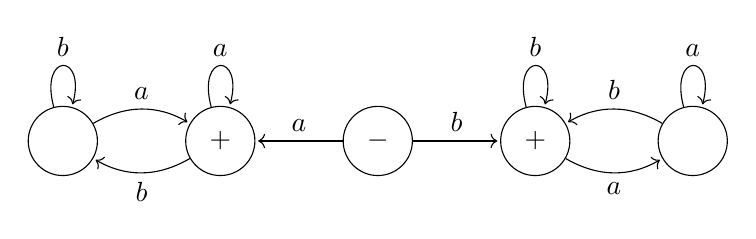
\begin{tikzpicture}[shorten >=1pt,node distance=2cm,on grid,auto] 
   \node[state] (q0)   {$-$}; 
   \node[state] (a1) [left=of q0] {$+$}; 
   \node[state] (a2) [left=of a1] {}; 
   \node[state] (b1) [right=of q0] {$+$}; 
   \node[state] (b2) [right=of b1] {}; 
   % \node[state,accepting](q_3) [below right=of q_1] {$q_3$};
    \path[->] 
      (q0) edge node [swap]{$a$} (a1)
      (a1) edge[loop above] node {$a$} (a1)
            edge[bend left] node {$b$} (a2)
      (a2) edge[bend left] node {$a$} (a1)
      edge[loop above] node {$b$} (a2)


      (q0) edge node {$b$} (b1)
      (b1) edge[loop above] node {$b$} (b1)
      edge[bend right] node [swap]{$a$} (b2)
      (b2) edge[bend right] node [swap]{$b$} (b1)
      edge[loop above] node {$a$} (b2)

    % (q_0) edge  node {0} (q_1)
    %       edge  node [swap] {1} (q_2)
    % (q_1) edge  node  {1} (q_3)
    %       edge [loop above] node {0} ()
    % (q_2) edge  node [swap] {0} (q_3) 
    %       edge [loop below] node {1} ();
      ;
\end{tikzpicture}
  \end{center}
  \caption{A finite state automaton.}\label{fig:2b}
\end{figure}

\section*{Question 3}
\begin{center}
  \textit{
    This question introduces the language $\big\{w\#w~\big|~w \in \{0,1\}^*\big\}$
    and asks whether it is regular.
  }
\end{center}
I think that it is not regular.

The pumping lemma gives us that a necessary condition for $L$
to be regular is: there exists $p_L \ge 1$ such that for every $w \in L$
where $\ell(w) > p_L$, there exists $x,y,z$ such that $w = xyz$ and 
(1) $\ell(y) \ge 1$, (2) $\ell(xy) \le p_L$, and (3) $xy^nz \in L$ for all $n \ge 0$.
We will prove the negation of this necessary condition.
%
That is,
for all $p_L \ge 1$,
there exists $w \in L$ such that $\ell(w) > p_L$ and,
for all decompositions,
at least one of the three decomposition properties
is violated.
This will show non-regularity by contraposition.

\begin{proof}[Proof \textrm{(Refutation of the necessary cond.)}.]
Let $p_L$ be arbitrary but fixed.
Choose $w = 0^{p_L}\#0^{p_L}$, noting that $w \in L$, and consider an arbitrary decomposition $w=xyz$.
Without loss of generality, assume $\ell(y) \ge 1$ and $\ell(xy) \le p_L$ (otherwise, at least one property is contradicted and we would be done).
% wlog, assume $\ell(xy) \le p_L$ (otherwise done).

Now, we consider where the hash character might have fallen in this decomposition.
If $y$ contains the hash, the final property is plainly false since words of $L$ have exactly one hash.
If $x$ contains the hash, then there is a fixed number of zeros to the left of the hash within $x$.
In this case, since $y$ is non-empty and to the right of the hash,
it contains at least one zero, and repeating $y$ would produce a word not in
$L$---negating the final property.
A symmetric argument holds for the $z$ case, and
% Therefore,
we find that the final property is unsatisfiable in the presence of the first two properties.
This is enough.
\end{proof}

\noindent And so it is shown.



\newpage
\section*{Question 4}
\subsection*{Question 4(a)}
\begin{center}
  \textit{
    This question wants to know the language recognised by a given Turing machine.
  }
\end{center}
Notice that the Turing machine has only edges of the form $x/x/\mathrm R$,
meaning the tape is never changed and the head is only moved right.
Since this machine never modifies memory and only scans the string once,
it acts just like a finite state automaton---specifically,
the FSA of Figure~\ref{fig:4a}.
This is mostly straightforward, with most edges being replaced with
with FSA edges of their recognised character.
Note that edges of the form $\emptyset/\emptyset/\mathrm R$
instead cause their source states to be marked as accepting states.

This makes it easier to infer the language (which is regular).
As a regular expression, this is
\begin{align*}
  \texttt{1$^*$ 0$^+$ 1$^+$ 0$^*$ ( 0 1$^+$ 0$^+$ 1$^+$ 0$^*$ )$^*$}.
  % (\texttt 0)^* \texttt 1 ( (\texttt 1)^* \texttt 0 (\texttt 1) ^* \texttt 0 )^*
\end{align*}
This language contains a number of repeating ``runs'' of 
\texttt{0}'s and \texttt{1}'s (a run is a contiguous block of one character).
Specifically, this language is the language of binary strings such that
after the first zero, they contain an \textit{odd} number of \texttt 1 runs.
There may or may not be a run of \texttt 1's before the first zero,
and there may or may not be a run of \texttt 0's after the last one.

By noticing the repetition in the above regular expression, this can also be seen as
\begin{align*}
  A\texttt{ ( 01 $A$ )}^*
  \textrm{\quad{}where\quad{}}A = \texttt{( 1$^*$ 0$^+$ 1$^+$ 0$^*$ )}.
  % (\texttt 0)^* \texttt 1 ( (\texttt 1)^* \texttt 0 (\texttt 1) ^* \texttt 0 )^*
\end{align*}
That is, a sequence of one or more \texttt{01}-separated
words in $A$, where $A$ is made up of
words containing a core of a \texttt 0 run then a \texttt 1 run, possibly prefixed by a \texttt 1 run or suffixed by a \texttt 0 run.


\begin{figure}
  \begin{center}
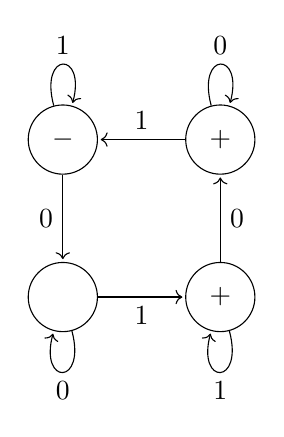
\begin{tikzpicture}[shorten >=1pt,node distance=2cm,on grid,auto] 
   \node[state] (q0)   {$-$}; 
   \node[state] (q1) [below=of q0] {}; 
   \node[state] (q2) [right=of q1] {$+$}; 
   \node[state] (q3) [above=of q2] {$+$}; 
    \path[->] 
    (q0) edge [loop above] node {1} (q0)
    (q0) edge node [swap]{0} (q1)
    (q1) edge [loop below] node {0} (q1)
    (q1) edge  node[swap] {1} (q2)
    (q2) edge  [loop below] node {1} (q2)
    (q2) edge   node[swap] {0} (q3)
    (q3) edge [loop above] node {0} (q3)
    (q3) edge  node[swap] {1} (q0)

    % (q_0) edge  node {0} (q_1)
    %       edge  node [swap] {1} (q_2)
    % (q_1) edge  node  {1} (q_3)
    %       edge [loop above] node {0} ()
    % (q_2) edge  node [swap] {0} (q_3) 
    %       edge [loop below] node {1} ();
      ;
\end{tikzpicture}

  \end{center}
  \caption{A finite state automaton.}\label{fig:4a}
\end{figure}


\newpage
\subsection*{Question 4(b)}
\begin{center}
  \textit{
    This question asks  (boldly) for a Turing machine to recognise the language of Question 3.
  }
\end{center}
Recall that the language is
$\{w\#w~|~w \in \{0,1\}^*\}$.
This will be done with the help of some basic Turing machine primitives to manipulate the tape. These are given (in pseudocode)
in Figure~\ref{fig:tm1}, and the main procedure is in Figure~\ref{fig:tm2}.
Initially, the head points to the leftmost character of the candidate string.
The algorithm then proceeds recursively, checking one character at a time:
\begin{enumerate}[label=(\arabic*),noitemsep]
  \item If the head character is a \texttt{\#}, ensure the string is precisely `\texttt{\#}'---if so, accept, else reject.
  \item If the head character is a \texttt{0} or \texttt 1, record this character as $c$, clear the tape position, then:
    \begin{enumerate}[noitemsep]
      \item Scan right until \texttt{\#}, then ensure the character right of \texttt{\#} matches $c$.
      \item Shuffle remaining string one position to the left,
        overwriting the just-checked character.
      \item Scan far left until the beginning of the string is reached,
        recalling that the original leftmost character was deleted
        so our string has become shorter.
      \item Repeat from (1).
    \end{enumerate}
\end{enumerate}
The Turing machine is depicted in Figure~\ref{fig:tm}.
This is a fairly faithful translation of the pseudocode.
Note that each \texttt{left\_until}/\texttt{right\_until} call appears as a single looping state (marked with $\leftarrow$/$\rightarrow$),
and the \texttt{shift\_left} routine's states are marked by $\ll$.

\begin{figure}

\begin{minted}[escapeinside=@@,frame=single,framesep=8pt,fontsize=\footnotesize]{python}
def left_until[Marker]():
  """ output with Marker=0: (0) A B C D ... """
  while True:
    if tape(Marker, Marker, R): break
    elif tape(0, 0, L) or tape(1, 1, L): continue
  assert tape(_, _, L)  # unconditionally move left
def right_until[Marker]():
  """ output with Marker=0: ... A B C D (0) """
  while True:
    if tape(Marker, Marker, L): break
    elif tape(0, 0, R) or tape(1, 1, R): continue
  assert tape(_, _, R)

def shift_left():
  """
  input:   X  0  A  B  A (B) 0
  output: (X) A  B  A  B  0  0
  """
  def shl_1():
    if tape(1, 1, L): shl_1()
    elif tape(0, 1, L): shl_0()
    elif tape(None, 1, L): return
  def shl_0():
    if tape(1, 0, L): shl_1()
    elif tape(0, 0, L): shl_0()
    elif tape(None, 0, L): return

  if tape(0, None, L): shl_0()
  elif tape(1, None, L): shl_1()
  elif tape(None, None, L): return
\end{minted}
  \caption{Helper functions for a Turing machine.}\label{fig:tm1}
\end{figure}


\begin{figure}[h]

  \begin{minted}[frame=single,framesep=8pt]{python}
def main():
  while True:
    if tape('#', '#', R):
      assert tape(None, None, R), "spurious chars after #"
      accept()

    elif tape(0, None, R):
      right_until['#']()
      assert tape('#', '#', R)
      assert tape(0, None, R)
    elif tape(1, None, R):
      right_until['#']()
      assert tape('#', '#', R)
      assert tape(1, None, R)

    # now, pointing at head of tail: 0 (A) B A B 0
    right_until[None]()
    assert tape(None, None, L)

    # shuffle string after '#' to the left by one position
    shift_left()
    assert tape('#', '#', L)

    left_until[None]()
    assert tape(None, None, R)
\end{minted}

  \caption{Main functionality of Turing machine.}\label{fig:tm2}
\end{figure}

\begin{figure}[h]
  \begin{center}
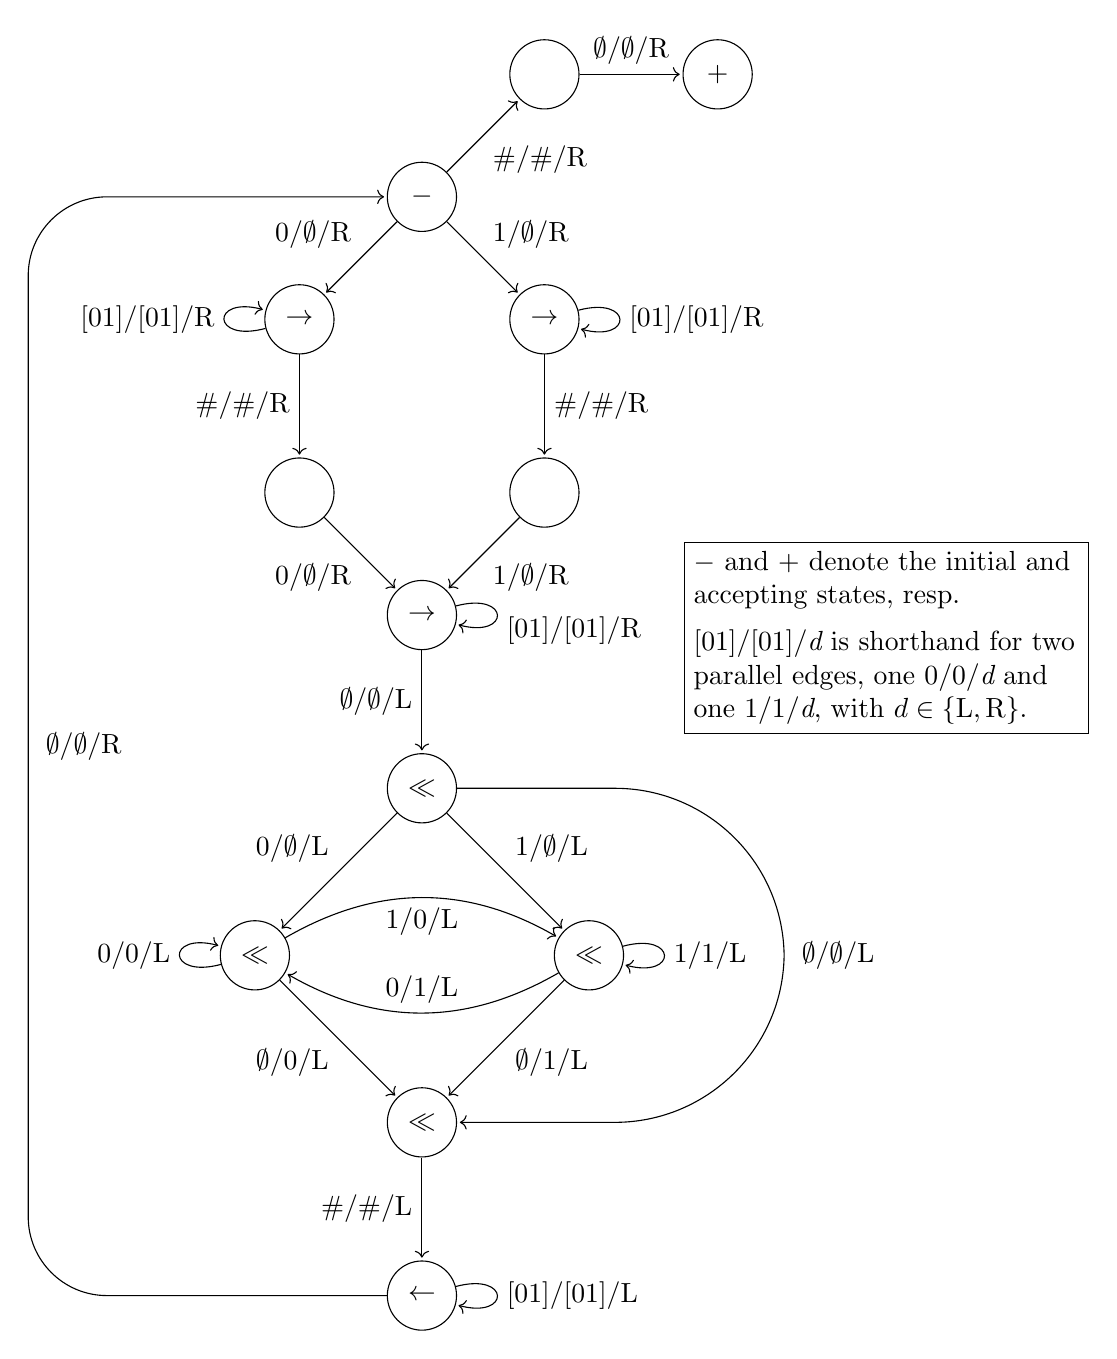
\begin{tikzpicture}[shorten >=1pt,node distance=2.2cm,on grid,auto] 

  \tikzset{
    rc/.style={rounded corners=2mm},
  }

   \node[state] (q0)   {$-$}; 
   \node[state] (qhash1) [above right=of q0] {}; 
   \path[->] (q0) edge node [swap]{$\#/\#/\mathrm R$} (qhash1);
   \node[state] (qhash2) [right=of qhash1] {$+$};
   \path[->] (qhash1) edge node {$\emptyset/\emptyset/\mathrm R$} (qhash2);

   % ZEROS

   \node[state] (qzero1) [below left=of q0]{$\rightarrow$};
   \path[->] (q0) edge node [swap]{$0/\emptyset/\mathrm R$} (qzero1);
   \path[->] (qzero1) edge [loop left] node {$[01]/[01]/\mathrm R$} (qzero1);


   \node[state] (qzerocheck) [below =of qzero1]{};
   \path[->] (qzero1) edge  node [swap]{$\#/\#/\mathrm R$} (qzerocheck);

   \node[state] (scanright) [below right=of qzerocheck] {$\rightarrow$};
   \path[->] (qzerocheck) edge node [swap]{$0/\emptyset/\mathrm R$} (scanright);

   \path[->] (scanright) edge [loop right] node [yshift=-0.2cm]{$[01]/[01]/\mathrm R$} (scanright);

   \node[state] (beginshift) [below =of scanright] {$\ll$};
   \path[->] (scanright) edge node [swap]{$\emptyset/\emptyset/\mathrm L$} (beginshift);

   \node[state] (ones) [below right=3cm of beginshift] {$\ll$};
   \path[->] (beginshift) edge node {$1/\emptyset/\mathrm L$} (ones);
   \node[state] (zeros) [below left=3cm of beginshift] {$\ll$};
   \path[->] (beginshift) edge node [swap]{$0/\emptyset/\mathrm L$} (zeros);

   \path[->] (ones) edge [bend left] node [swap]{$0/1/\mathrm L$} (zeros);
   \path[->] (ones) edge [loop right] node {$1/1/\mathrm L$} (ones);
   \path[->] (zeros) edge [bend left] node [swap]{$1/0/\mathrm L$} (ones);
   \path[->] (zeros) edge [loop left] node {$0/0/\mathrm L$} (zeros);


   \node[state] (endshift) [below right=3cm of zeros] {$\ll$};
   \path[->] (zeros) edge  node [swap]{$\emptyset/0/\mathrm L$} (endshift);
   \path[->] (ones) edge  node {$\emptyset/1/\mathrm L$} (endshift);
   % \path[->] (beginshift) edge[bend left=4cm] node
   % [swap]{$\emptyset/\emptyset/\mathrm L$} (endshift);

   \draw [->,rounded corners=2.15cm](beginshift) to
   ($(beginshift)+(4.6, 0)$) to   node[xshift=0.1cm]{$\emptyset/\emptyset/\mathrm L$}($(endshift)+(4.6,0)$) to  (endshift);

   \node[state] (hashagain) [below=of endshift] {$\leftarrow$};
   \path[->] (endshift) edge node [swap] {$\#/\#/\mathrm L$} (hashagain);
   \path[->] (hashagain) edge [loop right] node  {$[01]/[01]/\mathrm L$} (hashagain);

   % \node (leftmarker1) [left=3cm of hashagain,scale=0pt] {};
   % \node (leftmarker2) [left=3cm of q0] {};
   % \path[-] (hashagain) edge  node  {asdf} (leftmarker1);
   % \path[-] (leftmarker1) edge node {} (leftmarker2);
   \draw [->,rounded corners=1cm](hashagain) to
   ($(hashagain)+(-5, 0)$) to   node[swap,xshift=0.1cm]{$\emptyset/\emptyset/\mathrm R$}($(q0)+(-5,0)$) to  (q0);
   % \path[->] (hashagain) edge [bend left=16cm] node {asd} (q0);




   % ONES

   \node[state] (qone1) [below right=of q0]{$\rightarrow$};
   \path[->] (q0) edge node {$1/\emptyset/\mathrm R$} (qone1);
   \path[->] (qone1) edge [loop right] node {$[01]/[01]/\mathrm R$} (qone1);
   \node[state] (qonecheck) [below =of qone1]{};
   \path[->] (qone1) edge  node {$\#/\#/\mathrm R$} (qonecheck);
   \path[->] (qonecheck) edge  node {$1/\emptyset/\mathrm R$} (scanright);

  \node[draw,align=left,text width=4.9cm] at (5.9,-5.6) {
    $-$ and $+$ denote the initial and accepting states, resp. \\[0.5em]
    $[01]/[01]/\textit{d}$ is shorthand for two parallel edges,
    one $0/0/\textit{d}$ and one $1/1/\textit{d}$,
    with $d \in \{\mathrm L,\mathrm R\}$.
  };



    % (q_0) edge  node {0} (q_1)
    %       edge  node [swap] {1} (q_2)
    % (q_1) edge  node  {1} (q_3)
    %       edge [loop above] node {0} ()
    % (q_2) edge  node [swap] {0} (q_3) 
    %       edge [loop below] node {1} ();
\end{tikzpicture}

  \end{center}
  \caption{A Turing machine.}\label{fig:tm}
\end{figure}

% \clearpage
% Let's not do that again.

\end{document}

